\documentclass[11pt]{article}

\usepackage[a4paper,margin=0.9in]{geometry}
\usepackage{graphicx}
\usepackage{booktabs}
\usepackage{amsmath}
\usepackage{hyperref}
\usepackage{xcolor}
\usepackage{caption}
\usepackage{enumitem}
\setlist{nosep}

\title{\textbf{RuleTrace Scholar}: Explainable Agentic RAG\\ with Adaptive Evidence Rules}
\author{}
\date{\today}

\begin{document}
\maketitle
\vspace{-1.2em}

\begin{abstract}
\noindent I present \textbf{RuleTrace Scholar}, an explainable multi-agent retrieval-augmented generation (RAG) system for academic papers. The system combines (i) structure-aware PDF parsing; (ii) BM25--dense hybrid retrieval with cross-encoder reranking, metadata-aware evidence diversification, and parent expansion; (iii) a LangGraph pipeline that decomposes questions and dispatches reflective sub-agents; (iv) lazy vision--language grounding for figures; and (v) TRACE, a deterministic explanation layer that maps answer claims to retrieved evidence and evaluates adaptive grounding, validity, traceability, diversity, and density rules. TRACE exports every rule activation, an uncalibrated evidence-quality index, a risk decision, and counterfactual retrieval actions. This design provides evidence-path interpretability without claiming that the underlying language model is intrinsically interpretable.
\end{abstract}

\vspace{-0.6em}
\section{Introduction}
\vspace{-0.3em}
Academic readers often need to answer questions that span \emph{multiple sections} of a paper, \emph{multiple papers}, or \emph{non-textual elements} such as tables and figures. Vanilla RAG (flat chunking + single-shot dense retrieval + one-shot generation) struggles in this setting: (1) PDF structure is lost during naive extraction, so section- and figure-level context is unrecoverable; (2) a single retrieval pass cannot satisfy multi-hop or comparative queries; and (3) answers grounded in charts or architecture diagrams require visual understanding that text-only pipelines cannot provide.

\textbf{RuleTrace Scholar} retains this agentic pipeline but treats a citation list as insufficient explanation. After synthesis, TRACE segments the answer into factual claims, connects each claim to the exact retrieved evidence it cites, and applies question-dependent evidence rules. The same provenance used during generation therefore drives the exported explanation and release decision. This report describes the architecture (Sec.~\ref{sec:arch}), the key techniques (Sec.~\ref{sec:methods}), and the evaluation plan (Sec.~\ref{sec:eval}).

\vspace{-0.4em}
\section{System Architecture}
\label{sec:arch}
\vspace{-0.3em}

RuleTrace Scholar has three phases: an \emph{offline ingestion} pipeline that converts PDFs into a structured vector store, an \emph{online agent} pipeline that answers user queries, and a \emph{TRACE evidence audit} that produces the claim graph and reliability decision. Figure~\ref{fig:pipeline} summarizes the inherited ingestion and agent flow; TRACE follows synthesis and is exposed in the answer interface.

\begin{figure}[t]
\centering
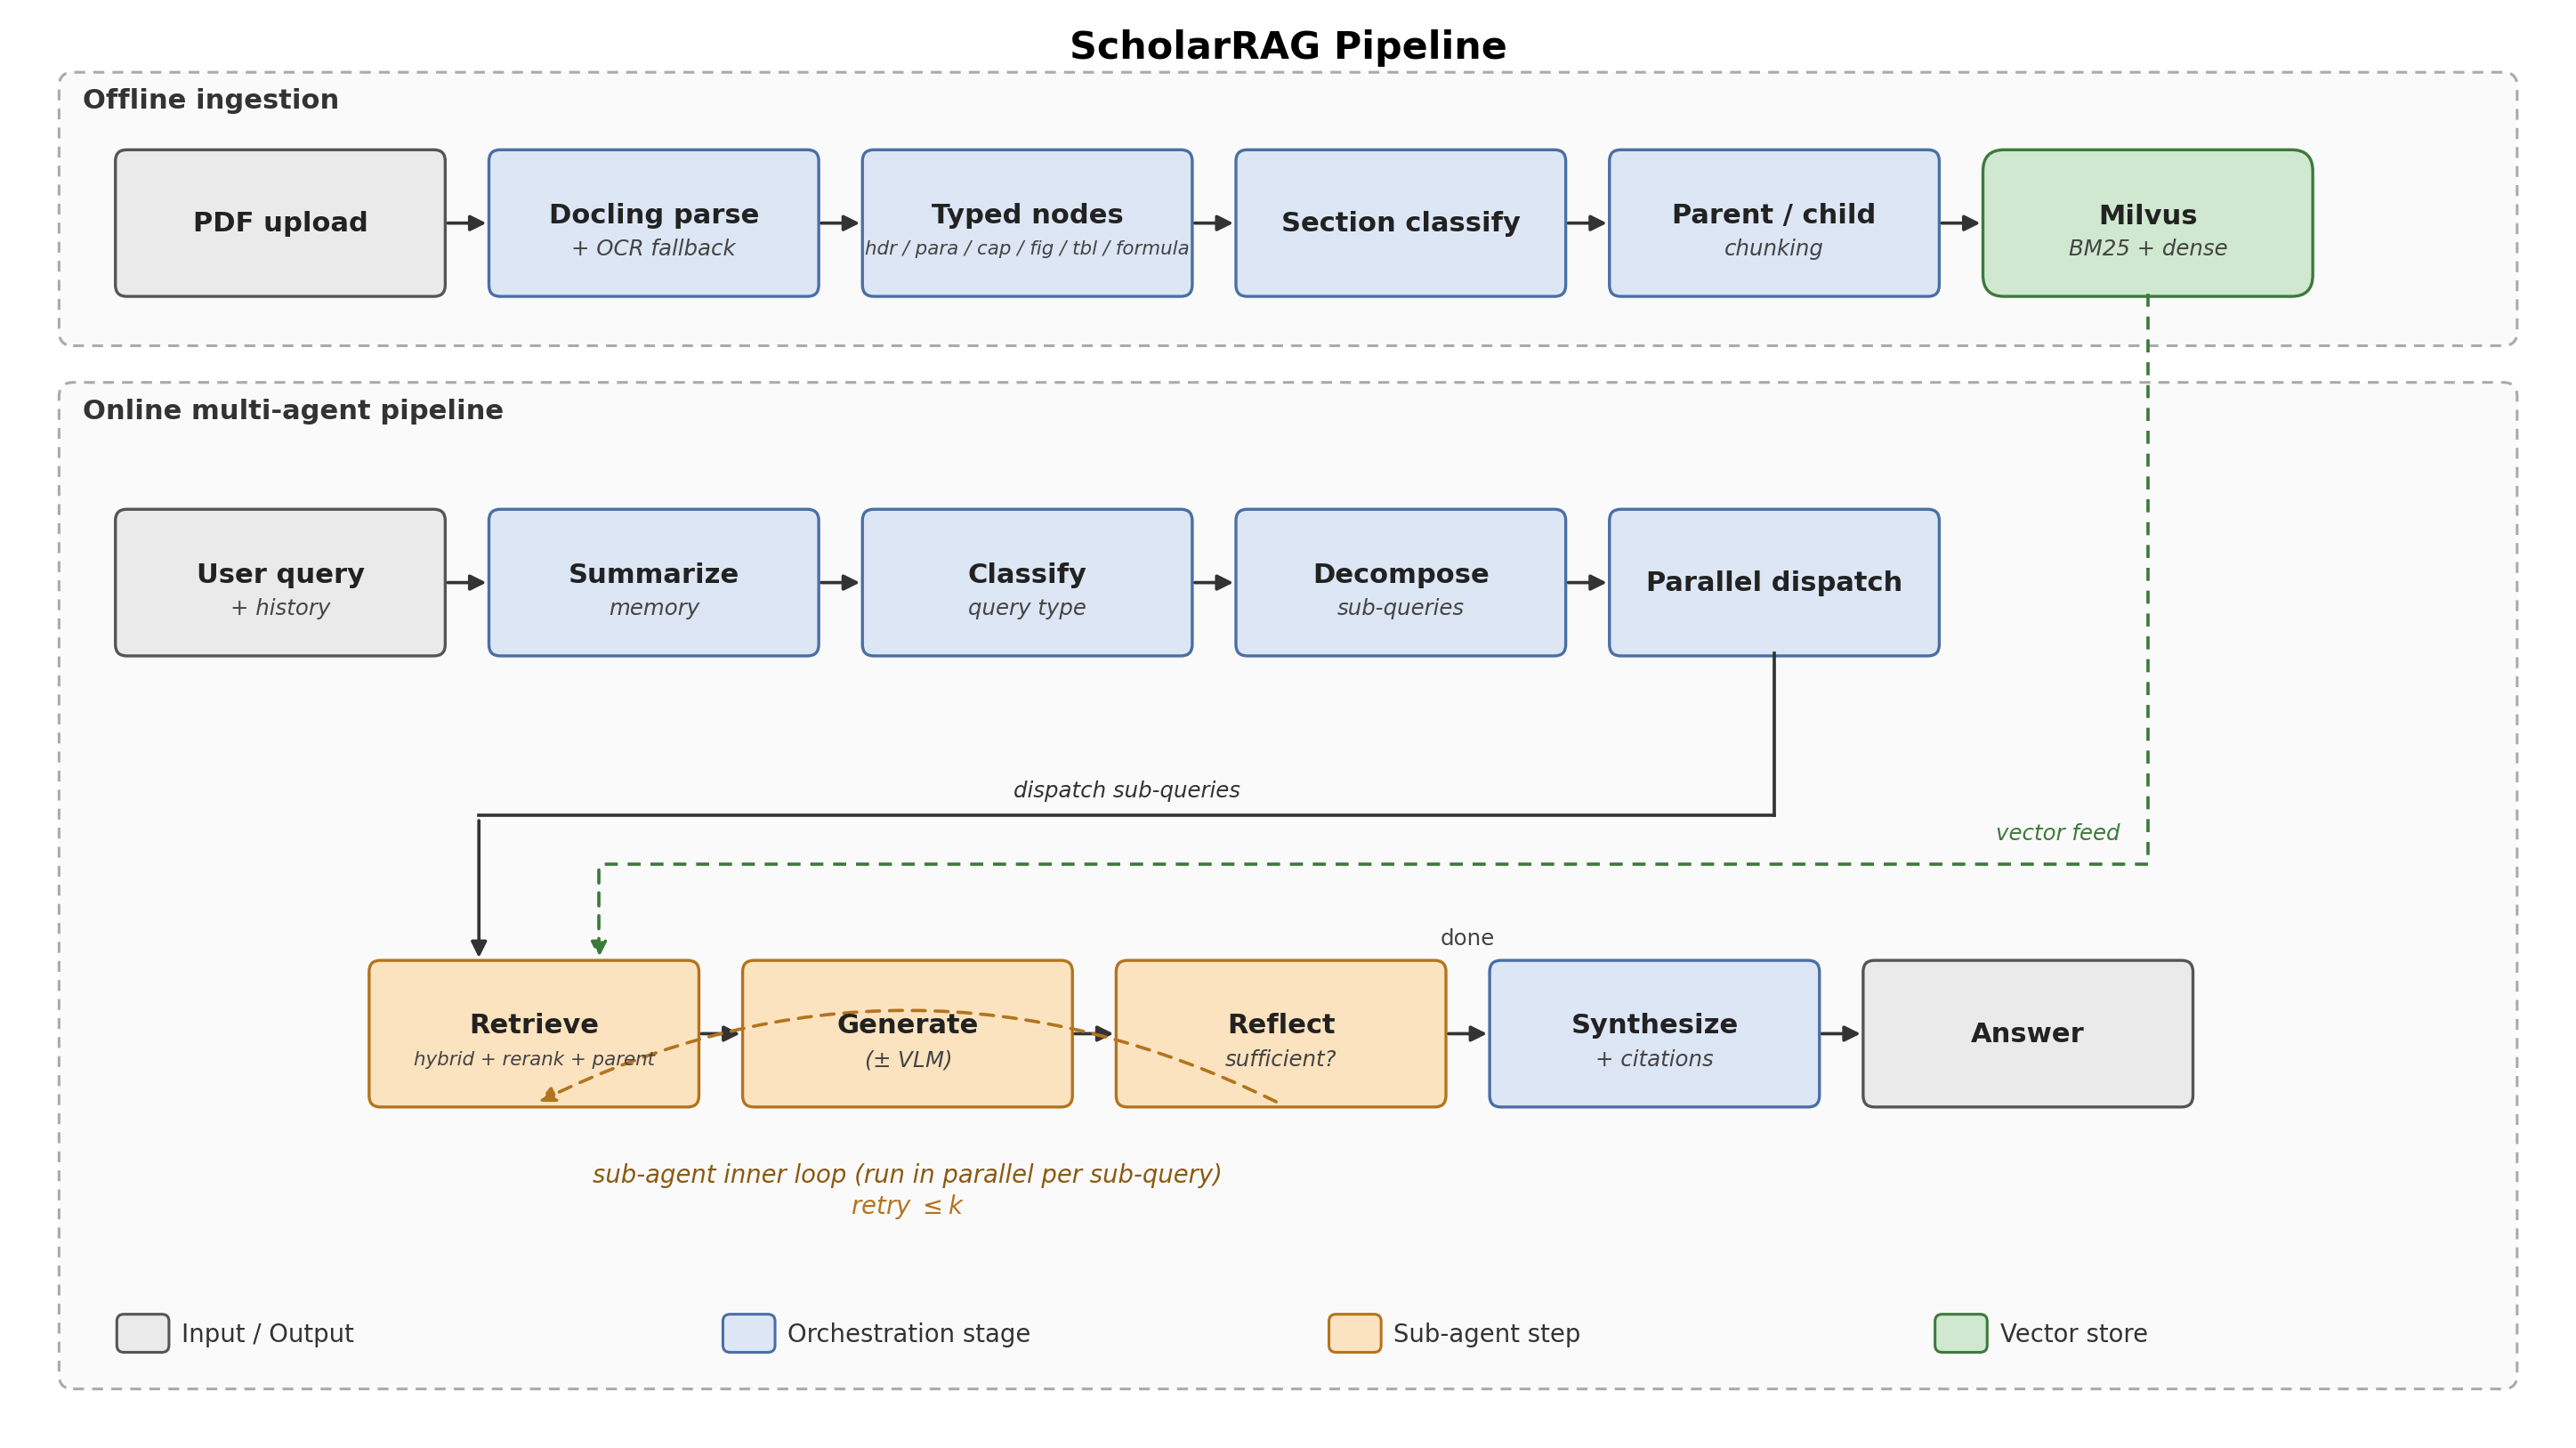
\includegraphics[width=\linewidth]{doc/pipeline.png}
\caption{Base ingestion and agent pipeline. RuleTrace Scholar adds evidence diversification before parent expansion and applies TRACE claim--evidence auditing after synthesis.}
\label{fig:pipeline}
\end{figure}

\paragraph{Main graph.} The top-level graph follows \texttt{START $\to$ summarize $\to$ classify $\to$ analyze $\to$ (sub\_agent $\times N$) $\to$ prepare\_synthesis $\to$ END}. The \texttt{summarize} node implements a sliding-window + LLM-summary memory: the last $W{=}6$ messages are kept verbatim while older turns are compressed into a rolling summary and persisted through a Postgres checkpointer, so long sessions do not blow up the prompt.

\paragraph{Sub-agent graph.} Each decomposed sub-query is dispatched via LangGraph's \texttt{Send} primitive to an independent sub-agent with its own state. A sub-agent runs \texttt{retrieve $\to$ generate $\to$ reflect}, and a conditional edge sends it back to \texttt{retrieve} (with a refined query) if reflection judges the answer insufficient, up to \texttt{max\_retries}. Sub-answers are merged into a global citation list that is re-indexed before synthesis.

\vspace{-0.3em}
\section{Methodology}
\label{sec:methods}
\vspace{-0.2em}

\subsection{Structure-Aware PDF Ingestion}
PDFs are parsed by \textbf{Docling} into typed items which I normalize into six node types (\texttt{section\_header}, \texttt{paragraph}, \texttt{caption}, \texttt{figure}, \texttt{table}, \texttt{formula}). Each node carries a \emph{section path} (e.g.\ \textit{Experiments~$\triangleright$~Ablation}), page number, bounding box, and order. Three pre-processing steps make downstream retrieval more robust: (i) \textbf{noise filtering}---headers, footers, and page numbers are removed using bounding-box heuristics (top/bottom 10\% of the page); (ii) \textbf{reading-order recovery}---items are grouped into rows using a per-page tolerance derived from average line height, then sorted top-to-bottom and left-to-right, which handles single- and two-column layouts uniformly; (iii) \textbf{OCR fallback}---if text density is below a threshold ($<$1000 chars total or $<$200 chars/page), Docling is re-invoked with OCR enabled.

Captions are then linked to their nearest figure/table, and an LLM classifies each section title into \{\texttt{method}, \texttt{experiment}, \texttt{background}, \texttt{conclusion}\}. Figure crops are saved to disk so that the VLM branch can analyze them on demand. Each node is turned into retrievable text by a \emph{type-specific content generator}: paragraphs are prefixed with their section path, tables are linearized into key-value rows (\texttt{Row $i$: $h_1{=}v_1, h_2{=}v_2, \dots$}), and figures are represented by their caption plus nearby textual context. Nodes are split into \emph{parent} chunks (large, for generation context) and \emph{child} chunks (small, for retrieval precision); both are embedded with BGE-small and stored in separate Milvus collections alongside BM25 sparse vectors.

\subsection{Hybrid Retrieval with Rerank and Parent Expansion}
Given a sub-query, retrieval executes
\[
\text{query} \xrightarrow{\text{(HyDE)}} \text{BM25+Dense} \xrightarrow{\text{RRF}} \text{CrossEncoder} \xrightarrow{\text{diversify}} \text{parent expand} \xrightarrow{} \text{Top-}K.
\]
Sparse (BM25) and dense (BGE) scores are fused with Reciprocal Rank Fusion inside Milvus, over-fetching $2\!\times\!\texttt{fetch\_k}$ candidates on the \emph{child} collection. A BGE cross-encoder (\texttt{bge-reranker-v2-m3}) then rescores the shortlist. A metadata-aware MMR step balances relevance with text novelty and rewards previously unseen papers and sections. Child hits are expanded to their parent chunks via the stored \texttt{chunk\_parent\_id}, yielding context windows large enough for coherent generation while retaining the precision of small-chunk retrieval. Optional HyDE rewriting is available for very short queries.

Retrieval is also \emph{routed} by query type: classification in the main graph (\{\texttt{experimental\_result}, \texttt{method}, \texttt{background}, \texttt{general}\}) is mapped to a Milvus filter on \texttt{section\_type}, so that result-oriented questions preferentially hit \textit{Experiments} sections. A fallback disables the filter if the constrained search returns empty.

\subsection{Agentic Reasoning: Decompose, Retrieve, Reflect, Synthesize}
Given a user query, the agent first runs \emph{classification} and \emph{decomposition} (structured-output LLM calls producing a \texttt{query\_type} and a list of \texttt{sub\_queries}, with the original query always kept as the first element). Sub-queries are dispatched in parallel; each sub-agent executes its own retrieve--generate--reflect cycle. The \textbf{reflection} step is an LLM that judges whether the generated answer is sufficient and, if not, proposes refined retry queries. A bounded retry counter (default 2) prevents unbounded loops. When all sub-agents finish, \texttt{prepare\_synthesis} concatenates sub-answers, remaps local citation indices \texttt{[1], [2], \dots} into a \emph{global} numbering, and hands the bundle to the synthesizer LLM, which produces the final answer while preserving citation tags.

\subsection{Lazy Vision--Language Grounding}
Because running a VLM on every figure is expensive, VLM analysis is invoked \emph{lazily} by a gating function: (i) \textbf{pre-generation}---the query contains visual keywords (\textit{figure, chart, plot, diagram}, \dots) and retrieval returned at least one figure node with an image path; (ii) \textbf{post-hoc (reflection) fallback}---the textual answer contains insufficiency phrases (e.g.\ \textit{``not contain sufficient information''}) and figure nodes are available; at most two figures are analyzed to bound cost. In both cases the VLM returns a structured description (chart type, axes, key trends, numerical values) which is appended to the context and the answer is re-generated. VLM descriptions are cached on citation metadata to avoid recomputation within a session.

\subsection{Multi-Turn Memory and Citations}
Conversation state is stored via LangGraph's Postgres checkpointer, keyed by session id. The \texttt{summarize} node maintains a rolling summary of all messages older than the last six turns, while the last six are injected verbatim into the system prompt as \texttt{<recent\_conversation>}. Citation metadata (\texttt{paper\_id}, \texttt{section\_path}, \texttt{page\_num}, \texttt{node\_type}, retrieval relevance, and an evidence excerpt) travels with each retrieved document. Internal image paths are removed before citations are persisted or returned to the client.

\subsection{TRACE Claim--Evidence Rules and Uncertainty}
Let $C=\{c_i\}$ be factual claims extracted from the final answer and $E=\{e_j\}$ the retrieved evidence items. A directed edge $c_i\rightarrow e_j$ exists only when the answer contains a valid citation index that resolves to $e_j$. TRACE computes five observable metrics: claim citation coverage $m_1$, citation-index validity $m_2$, provenance traceability $m_3$, source/section diversity $m_4$, and evidence density $m_5$. Each metric activates a rule
\[
r_k=\mathbb{I}\!\left[m_k\ge \tau_k(q,n)\right],
\]
where the threshold depends on query type $q$ and the number of decomposed sub-queries $n$. Quantitative result questions receive the strictest base thresholds, and complex questions increase the coverage, diversity, and release requirements.

The exported evidence-quality index is a transparent weighted sum with a failed-rule penalty:
\[
s=\left(\sum_{k=1}^{5}w_km_k\right)\left(0.85+0.15\frac{\sum_k r_k}{5}\right),
\qquad u=1-s.
\]
The UI displays $s$, the uncertainty index $u$, every $m_k$, threshold $\tau_k$, activation $r_k$, the claim--evidence graph, and actions that would flip failed rules. Because $s$ has not yet been fitted against labelled correctness outcomes, it is explicitly reported as an \emph{uncalibrated evidence-quality index}, not a truth probability.

\vspace{-0.3em}
\section{Evaluation}
\label{sec:eval}
\vspace{-0.2em}
I evaluate RuleTrace Scholar along three axes: \emph{retrieval quality}, \emph{generation quality}, and \emph{explanation quality} (does the exported trace faithfully and usefully expose the actual evidence path?).

\paragraph{Retrieval metrics.} On a chunk-level benchmark I compute Recall@$k$, Precision@$k$, Mean Reciprocal Rank (MRR), and Mean Average Precision (MAP) for $k\in\{1,3,5,10\}$. An adapter is also provided for the page-level MMDocIR benchmark, which matches retrieved documents to gold pages via a \texttt{hit\_fn}. Table~\ref{tab:retrieval} reports per-configuration numbers; ablations isolate the contribution of each retrieval component.

\begin{table}[h]
\centering
\small
\caption{Retrieval evaluation (custom benchmark, $k{=}5$). Numbers to be filled in.}
\label{tab:retrieval}
\begin{tabular}{lcccc}
\toprule
Configuration & Recall@5 & Precision@5 & MRR & MAP \\
\midrule
Dense only                                  & TBD & TBD & TBD & TBD \\
BM25 only                                   & TBD & TBD & TBD & TBD \\
Hybrid (BM25 + Dense + RRF)                 & TBD & TBD & TBD & TBD \\
\;\; + Cross-encoder rerank                 & TBD & TBD & TBD & TBD \\
\;\; + Parent expansion                     & TBD & TBD & TBD & TBD \\
\;\; + Evidence diversity                   & TBD & TBD & TBD & TBD \\
\;\; + Section-type routing (full)          & TBD & TBD & TBD & TBD \\
\bottomrule
\end{tabular}
\end{table}

\paragraph{Generation metrics.} I use RAGAS with four metrics: \emph{Faithfulness} (answer is grounded in retrieved context), \emph{Answer Relevancy}, \emph{Context Precision}, and \emph{Factual Correctness} (answer vs.\ reference). End-to-end samples are collected by invoking the full agent graph, so reported numbers reflect the combined effect of decomposition, reflection, and VLM. Table~\ref{tab:generation} reports RAGAS scores with and without key agent components.

\begin{table}[h]
\centering
\small
\caption{Generation evaluation (RAGAS). Numbers to be filled in.}
\label{tab:generation}
\begin{tabular}{lcccc}
\toprule
Configuration & Faith. & Ans.\ Rel. & Ctx.\ Prec. & Fact.\ Corr. \\
\midrule
Vanilla RAG (single retrieve + generate)        & TBD & TBD & TBD & TBD \\
\;+ Query decomposition                         & TBD & TBD & TBD & TBD \\
\;\;+ Reflection loop                           & TBD & TBD & TBD & TBD \\
\;\;\;+ VLM on visual queries (RuleTrace base) & TBD & TBD & TBD & TBD \\
\bottomrule
\end{tabular}
\end{table}

\paragraph{Explanation evaluation.} Structural metrics include citation coverage, reference validity, traceability, source diversity, evidence density, rule pass rates, and the distribution of guard decisions. A labelled study should additionally measure claim--evidence entailment, citation correctness, selective-risk curves, expected calibration error, and Brier score after calibration. Ablations compare fixed versus adaptive thresholds, retrieval with and without evidence diversification, citation-only UI versus TRACE, and deterministic rules versus LLM self-reported confidence. A user study should measure error acceptance, verification time, and over-trust.

\paragraph{Planned analyses.} I plan (i) a per-query-type breakdown; (ii) latency and token-cost accounting; (iii) semantic perturbation tests for claim, evidence, and rule stability; and (iv) qualitative failure analysis for unsupported claims, incorrect entailment, wrong figures, and over-decomposition.

\vspace{-0.3em}
\section{Discussion and Conclusion}
\vspace{-0.2em}
The agentic design buys quality and coverage but at a cost: each user turn can trigger $N$ parallel sub-agents, bounded retries, and optional VLM calls. Retrieval quality still depends on layout analysis, while citation presence alone cannot establish semantic entailment or causality. TRACE makes these boundaries visible and provides deterministic diagnostics, but its current score remains uncalibrated and must not be interpreted as answer correctness probability.

Overall, RuleTrace Scholar extends academic RAG with a reproducible evidence-path explanation layer: retrieve diversely, answer with local citations, expose claim--evidence edges, evaluate adaptive rules, and recommend counterfactual evidence actions. Future work will add evidence-level natural-language inference, stance graphs for genuine cross-paper contradictions, perturbation stability, and benchmark-based calibration.

\end{document}
